\chapter{Method}

\begin{enumerate}
  \item Description of Node Copying as a method
  \begin{enumerate}
    \item Node structure expansion
    \begin{enumerate}
      \item Back pointers
      \item Modifications
      \item Bounds on numbers of the above
      \item How it works
      \item Why it works
    \end{enumerate}
    \item Surrounding structure (collection of version information)
    \begin{enumerate}
      \item Considerations about effecient storage and retrieval of version info
    \end{enumerate}
  \end{enumerate}
  \item Description of ``Rollback'' as a method
  \item Description of reordering and optimization of operations
\end{enumerate}



This chapter should include:
\begin{itemize}
  \item Ensuring that the implementations of different approaches are fair
  \item Application profiles (modify-first, then access vs. mixed modify/access)
  \item Analysis what it costs having to know specifics of data structure to
  implement operation sequence pruning/optimization
\end{itemize}

\section{Rollback}

In the introduction section of \cite{Tsotras1995237} are described two basic,
na\"ive solutions to the query for $s(t)$, namely ``copy'' and ``log'':
\begin{description}
  \item[copy] works by storing a full copy of the data structure after each
  operation, thus allowing one to access any version simply by using the copy
  for the desired version. The obvious drawbacks of this approach is that space
  consumption can grow very fast. E.g. if only insertions are made, the cost is
  combinatorial $O\left(\binom{n+1}{2}\right)$ since every insertion will cost
  $O(1)$ more than the previous due to the growing size of each copy. On the
  other hand, access takes just $O(1)$.

  \item[log] works by storing a log of each operation made along with any
  information necessary to revert it. When a specific version is requested for
  access, operations can be applied or unapplied until the version is reached. 
  The obvious drawbacks for this approach are that access costs $O(n)$ in the 
  worst case, and if e.g. the initial, empty version has been accessed just 
  prior to a new operation being requested, the cost of that operation would 
  also be $O(n)$ since the whole log would have to be run through to produce 
  the latest version upon which the operation could be carried out. On the other
  hand, space consumption is $O(n)$ for $n$ operations.
\end{description}

An obvious improvement on both of the above approaches is to design a compound
data structure where copies are only made of a sub-set of the versions, and the
operations log is used to recreate any versions in between. The space
consumption would then become
$$O(n)+O\left(\binom{\left\lfloor{\frac{n+1}{d}}\right\rfloor}{2}\right)$$ where
$d$ is the distance between each full copy. Similarly, the time required to
recreate a specific version is in the worst case
$$O(1)+O\left(\frac{d}{2}\right)$$

The introduction of $d$ leads to the requirement of knowing a priori the
magnitude of the number of versions to expect. If $d$ is too small, space
consumption limits might be reached too early; if $d$ is too large, it may take
disproportionately long to recreate a desired version. A solution to this
problem is automatic scaling, i.e. increasing $d$ when space consumption is
nearing a given limit and possibly removing some data structure copies to
reflect the new value of $d$.

For large values of $d$ it is also worth considering the implementation details
of recreating the desired version using the operations log based on the
nearest full copy. If, for example, $d$ is 200, it would in the worst case be
necessary to work through 100 operations to reach the version which is exactly
in the middle of two full copies. Depending on the underlying data structure,
and the type and nature of the 100 operations, it can pay off to analyse,
prune and reorder the sequence of operations to reduce the number of I/O calls.
If, for example, the first 50 operations each insert an element, but the next 50
operations are deletions of those very same 50 elements, the entire sequence can
be reduced to a no-op, and the full copy can be presented as the answer to the
access query.

\subsection{Algorithm for optimization of operation batch}
\begin{algorithm}
  \caption{Pseudo-code for algorithm optimizing batch of operations}
  \begin{algorithmic}[1]
    %\Require current version $v_k$, desired version $v_d$
    \Function{OptimizeBatch}{current version $v_k$, desired version $v_d$}
      \State $O \gets \textsc{empty vector}$
      \For {each operation $o_i$ between $v_k$ and $v_d$}
        \If {$v_k<v_d$}
          \State push $o_i$ to back of $O$
        \Else
          \State push inverse of $o_i$ to back of $O$
        \EndIf
      \EndFor
      \For {each operation $o_i$ in $O$}
        \If {$o_i$ is an \textsc{insert} operation}
          \State $c \gets \textsc{index}(o_i)$
          \For {operation $o_j \in o_{i+1},\ldots$}
            \If {$o_j$ is an \textsc{insert} operation and \textsc{index}($o_j$)$<c$}
              \State $c \gets c+1$
            \ElsIf {$o_j$ is a \textsc{modify} operation and \textsc{index}($o_j$)$=c$}
              \State $\textsc{data}(o_i) \gets \textsc{data}(o_j)$
              \State $\textsc{delete}(o_j)$
              \State $\textsc{continue}\textnormal{ for loop with next }o_j$
            \ElsIf {$o_j$ is a \textsc{remove} operation}
              \If {\textsc{index}($o_j$) < c}
                \State $c \gets c-1$
              \ElsIf {\textsc{index}($o_j$) = c}
                \For {operation $o_k \in o_{i+1},\ldots,o_{j-1}$}
                  \State $\textsc{index}(o_k) \gets \textsc{index}(o_k) - 1$
                \EndFor
                \State $\textsc{delete}(o_i)$
                \State $\textsc{delete}(o_k)$
                \State $\textsc{continue}\textnormal{ for loop with next }o_i$
              \EndIf
            \EndIf
          \EndFor
        \EndIf
      \EndFor
      \Statex
      \State \textsc{sort}($O$) \{
      \State \hspace{12pt} \textsc{remove} op.s first by ascending index,
      \State \hspace{12pt} \textsc{modify},\textsc{insert} op.s last by descending index
      \State \}
      \Statex
      \State \Return $O$
    \EndFunction
  \end{algorithmic}
\end{algorithm}

\section{Node copying}
Node copying is described in \cite{Driscoll198986} and works by expanding the
existing data structure node. An array of field modifications of at least $p$ is
introduced which represents any modifications made to the node after its
creation. An array of so-called ``back pointers'' is maintained in node $x$
which contains a pointer to each node $y$ that contains a normal pointer to $x$.

Due to the assumption that the data structure has a bounded in-degree, these
arrays can be allocated statically, and thus assumptions can be made about the
space consumption per node.

See figure \ref{fig:pp-7-versions.pdf} for an illustrated example of the Node
Copying method.

If a modification is requested at a time when the modifications array is full, a
copy of the node is created with the most recent values for each field stored in
the original fields, and with an empty modifictations array. The back pointers
are inherited from the original node, and each node $y_i$ which back pointer
$x_i$ refers to is updated to point to the node copy. This can cause back
propagation, but the amortized cost has a constant upper bound.

\todo[inline]{Citation needed for back propagation cost amortization.}

\begin{figure}[!hbp]
    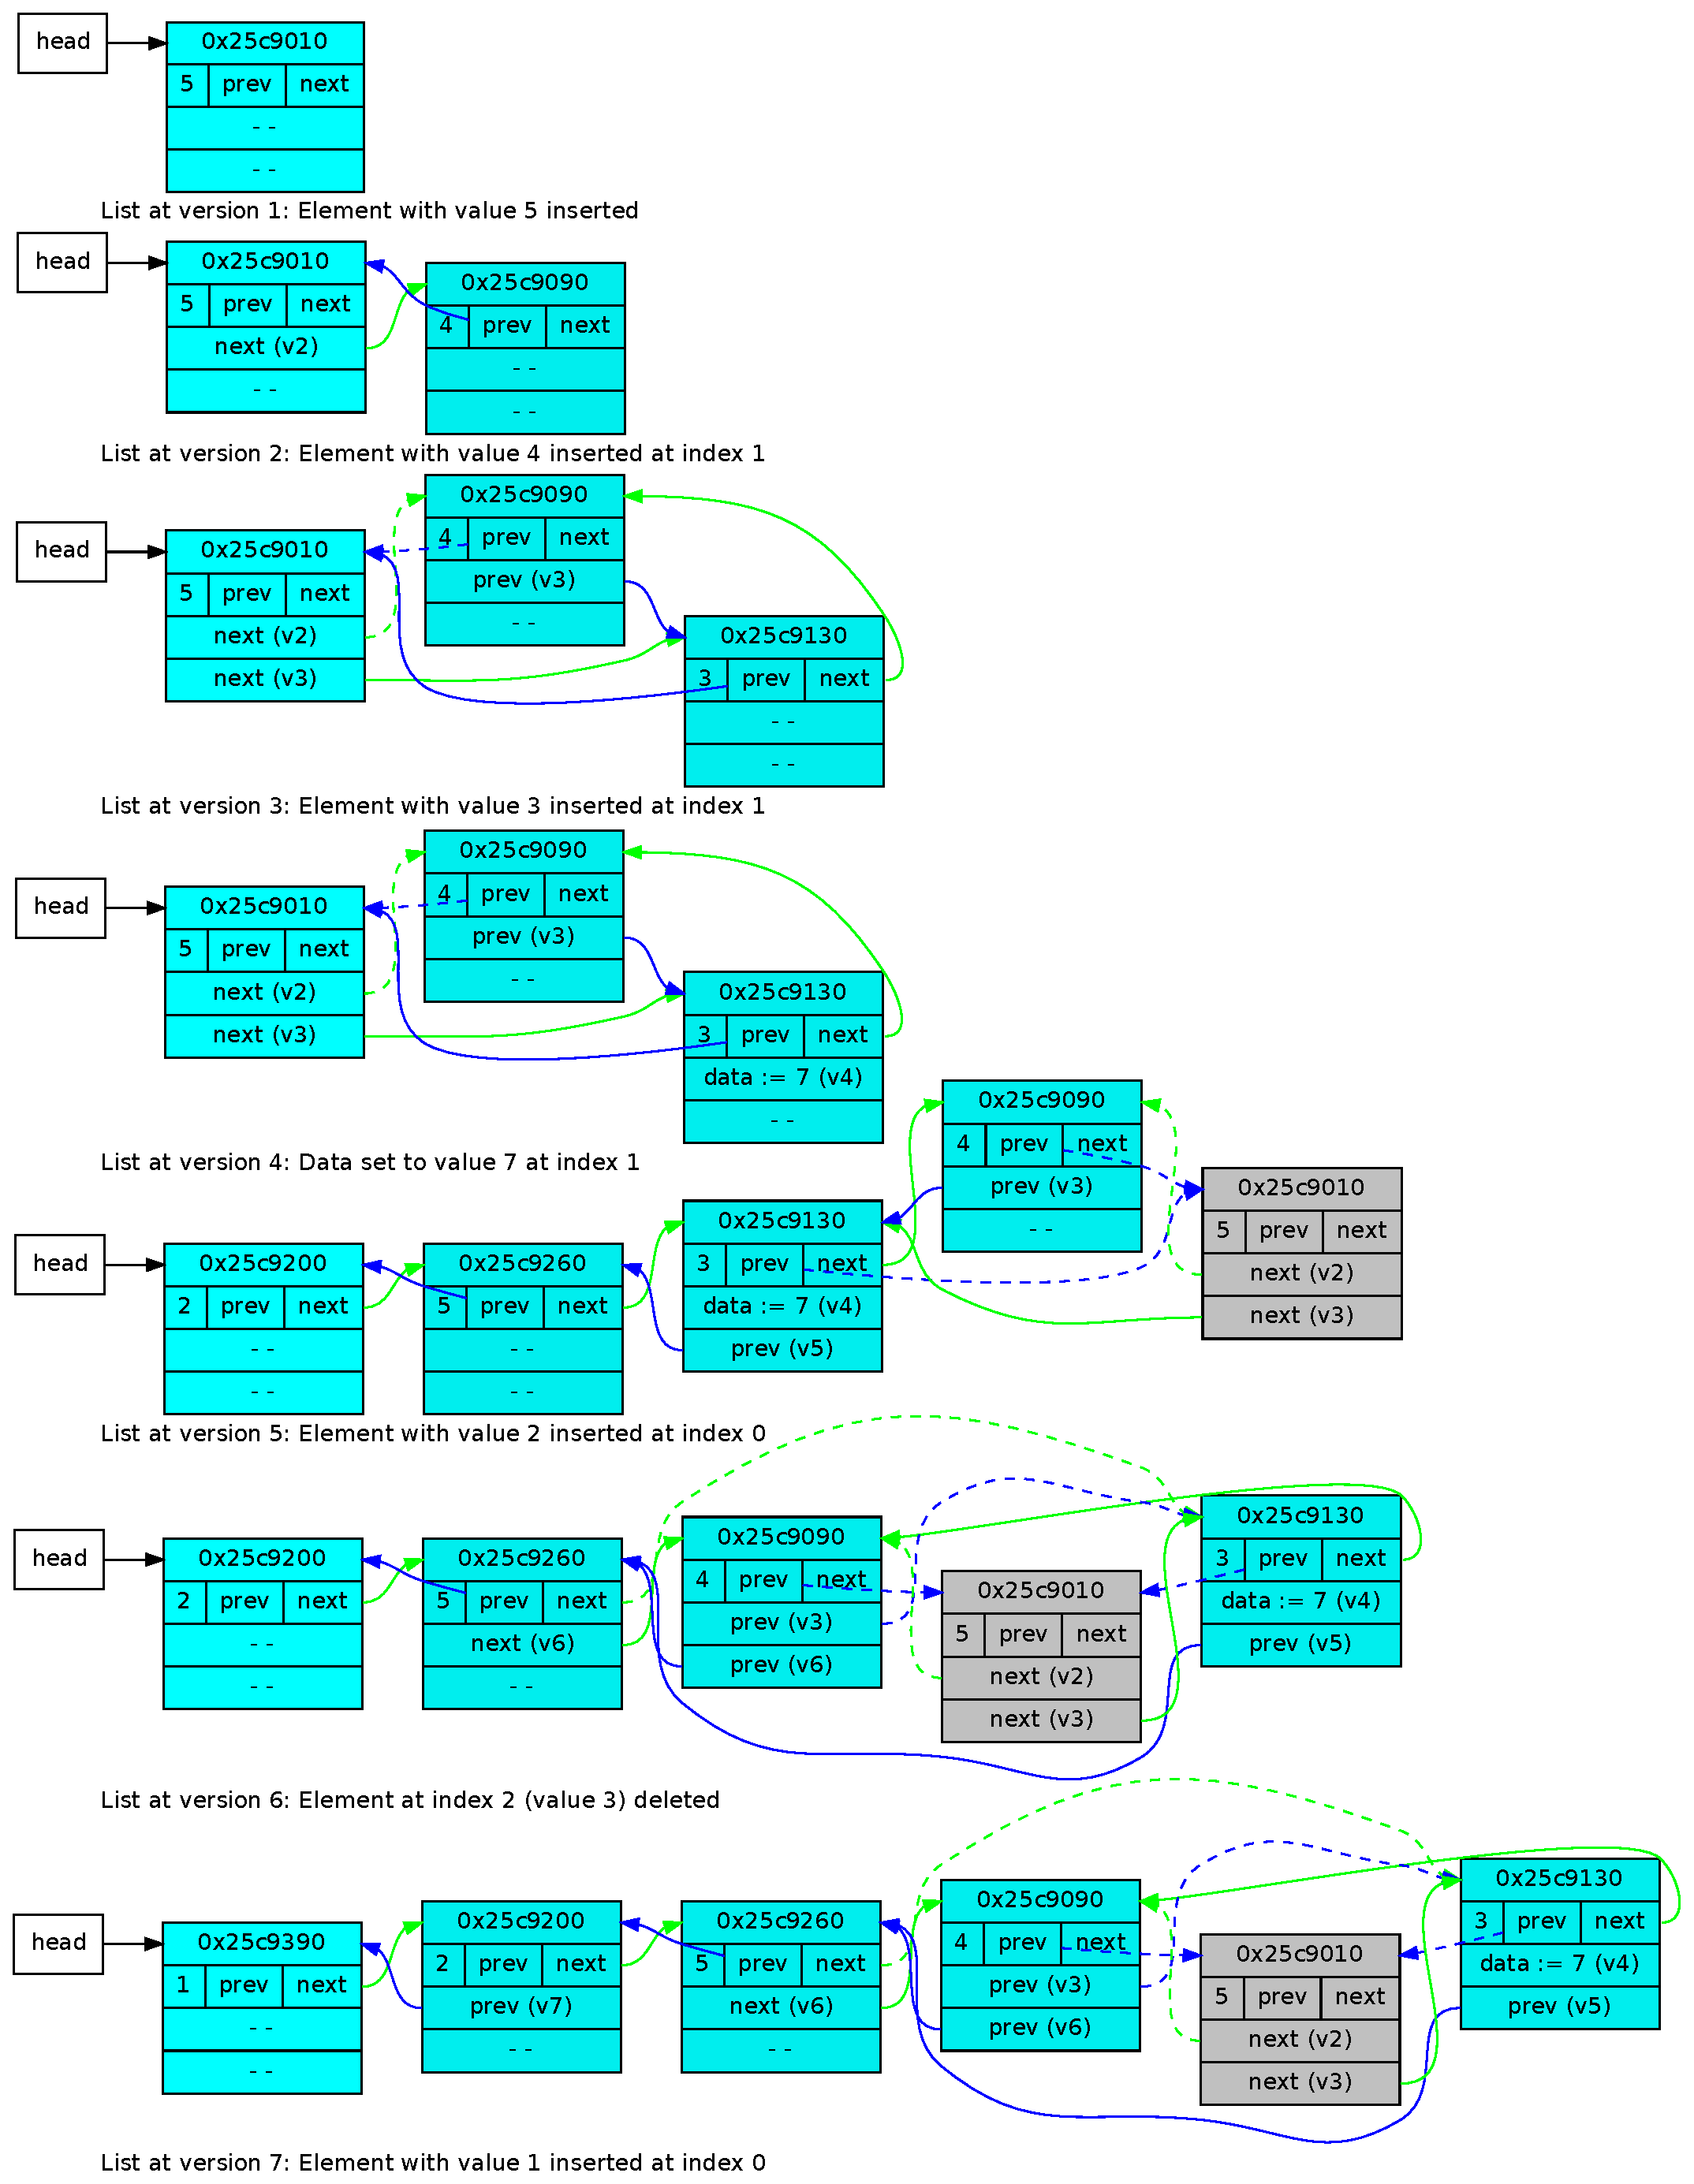
\includegraphics[width=\textwidth]{figures/pp-7-versions.pdf}
    \caption{7 versions of a doubly linked list made  partially persistent by
    the Node Copying method}
    \label{fig:pp-7-versions.pdf}
\end{figure}